\documentclass[conference]{IEEEtran}

\usepackage{graphicx}
\usepackage{subfig}
\usepackage{fixltx2e}

% correct bad hyphenation here
\hyphenation{op-tical net-works semi-conduc-tor}

\begin{document}

% paper title
\title{Growth, Diversity, and Evolution of Open Source IaaS Communities}

% author names and affiliations
% use a multiple column layout for up to three different
% affiliations
\author{
\IEEEauthorblockN{Qingye Jiang, Young Choon Lee, and Joseph G. Davis}
\IEEEauthorblockA{
Centre for Distributed and High Performance Computing\\
School of Information Technologies\\
The University of Sydney\\
Sydney NSW 2006, Australia\\
Email: qjiang@ieee.org, {young.lee, joseph.davis}@sydney.edu.au}
}

\maketitle


%abstract
\begin{abstract}
Community is an important aspect of open source projects in that it affects the perceived value of the project. In this paper, we study the user and developer communities of four major open source projects in the area of Infrastructure-as-a-Service (IaaS), namely, CloudStack, Eucalyptus, OpenNebula and OpenStack. We measure the size of the developer and user communities and model the growth of these communities using growth curves. We measure the activities of the developer and user communities and evaluate the contribution from the respective core contributor groups. Furthermore, we measure the diversity of the developer and user communities using Simpson's diversity index. We find out that communities with greater diversity exhibit closer-to-organic growth behavior and fit better with the growth curves. As well, communities with greater diversity are usually larger in terms of active membership.
\end{abstract}

\begin{IEEEkeywords}
open source software, cloud computing, community, growth curve, diversity index.
\end{IEEEkeywords}

\section{Introduction}
\label{sec:intro}

Community refers to a group of people having particular characteristics in common. In the case of open source software (OSS), a project's community includes the developers contributing code and the users consuming the code. During the past two decades, the information and communications technology (ICT) industry has witnessed a paradigm shift from traditional in-house software development model to an increased reliance on the open source development model. In the early days of the open source movement, open source was often described as a fundamentally new way to development software in that software is built by large number of volunteers working in an unorganized way in return for primarily intrinsic rewards. In recent years, we are observing an increasing number of organizations participating in the open source movement with the clear goal of pursuing commercial success. In particular, when a proprietary solution becomes successful in the market, there quickly appear one or more open source followers with similar features. The opposite case where open source solution comes before proprietary followers exists but is rare. When multiple open source projects are available in the same market segment, these projects compete with each other for market share. The result of such competition is often reflected in the changes in the size and activity in their communities.  
 
It is commonly agreed that the size of an open source community is associated with the market share of the project, and hence positively affects the perceived value of the project. However, there exists a knowledge gap concerning how open source communities rise and fall. Questions of great theoretical and practical importance include:

\begin{itemize}
	\item How to measure and describe the growth of open source communities?
	\item How important are the core contributors to the growth of open source communities? 
	\item How to measure the diversity of a community? How does diversity impact the growth of an open source community?
\end{itemize}

In this paper, we attempt to explore these questions using the developer and user communities of the major open source projects in the area of Infrastructure-as-a-Service (IaaS) as case studies. In enterprise data centers, deploying and managing large networks of virtual machines as scalable cloud computing platforms is largely supported by open source projects such as CloudStack, Eucalyptus, OpenNebula and OpenStack. We also present an analysis of the growth and evolution of the communities that underpin the ongoing development of these IaaS software. The results presented in this paper will enable open source vendors design better open source strategies leading to broader technology adoption and further market diffusion.

The rest of this paper is organized as follows. Section \ref{sec:projects} provides a brief description of the four open source projects being studied. Section \ref{sec:growth} introduces the concept of growth curves, and uses growth curves to model the growth of the developer and user communities. Section \ref{sec:activity} describes the activities in the developer and user communities, as well as characteristics of the core contributor group. Section \ref{sec:diversity} measures the diversity of the developer and user communities using Simpson's diversity index, with a discussion of the relationship between community diversity and growth. Section \ref{sec:related} describes related work. Our conclusions and the limitations of this study are presented in Section \ref{sec:conclusion}.

\section{Open Source IaaS Projects}
\label{sec:projects}

As defined by NIST \cite{nist}, IaaS is one of the three service models of cloud computing. It refers to the capability provided to the consumer to provision processing, storage, networking, and other fundamental computing resources where the consumer is able to deploy and run arbitrary software, including operating systems and applications. Amazon Web Services (AWS) are widely recognized as examples of public cloud services. Over the past years, the market witnessed a trend in developing new applications on AWS, or migrating existing applications to AWS. Inspired by the success of AWS, there emerge several open source projects trying to offer similar features. Among these projects, CloudStack, Eucalyptus, OpenNebula and OpenStack are the most popular ones.  

\begin{figure}[t!]
%\centering
 \subfloat[Normal Growth]{ 
    \label{fig:subfig:1a}  
    \includegraphics*[width=0.49\columnwidth,viewport=0 0 380 250]{6_fig01_a}} 
    \hspace{2pt}
  \subfloat[Bi-Phase Growths]{ 
    \label{fig:subfig:1b} 
    \includegraphics*[width=0.45\columnwidth,viewport=23 0 380 250]{6_fig01_b}} 
  \caption{Examples of Bacteria Growth Curves} 
  \vspace{-10pt}
  \label{fig:growth_bacteria} 
\end{figure}

CloudStack was developed by Cloud.com. The first open source version was released under the GNU General Public License, version 3 (GPLv3) in 2010. A proprietary enterprise edition with advanced features was released at the same time. In 2011 Citrix acquired Cloud.com and released the remaining code, which made CloudStack a complete open source project. In 2012 Citrix donated CloudStack to the Apache Software Foundation (ASF). As part of this change, Citrix changed the license of CloudStack to the Apache License, version 2. CloudStack completed the incubation phase and became a top-level project of ASF in early 2013.

Eucalyptus \cite{c1} started as a PhD dissertation project at the University of California at Santa Barbara. In 2009, a company with the same name was founded to commercialize the software. Originally, most of the software was released as Eucalyptus Community Edition under the Apache License, version 2. A proprietary enterprise edition with advanced features was released at the same time. In 2010, Eucalyptus changed the license of the open source part to GPLv2, but continued under the dual licensing model. In 2012, Eucalyptus dropped the dual licensing model, combined the original community and enterprise editions, and released a single open source version under GPLv2.

OpenNebula \cite{c2} was originally a research project at the Complutense University in Madrid, Spain. The first version was released in March 2008 under the Apache License, version 2. In 2010, the main authors of OpenNebula founded C12G Labs to provide value-added professional services around OpenNebula.

Rackspace and NASA co-founded the OpenStack project in 2010. The first version was released in 2010 under the Apache License, version 2. The early code came from NASA’s Nebula private cloud project \cite{c3}\cite{c4} and Rackspace’s cloud file service. The project quickly gained the attention from companies worldwide. As the number of participating entities continued to grow, the non-profit OpenStack Foundation was founded in 2012 to manage and promote OpenStack.

To study the growth of the developer communities, we collected data from the git repositories associated with these projects. All the four projects use git as their source code version control systems. In git, the entire history of a project is represented as a set of interrelated commits. We use git logs to retrieve information about each commit operation, including date and time of the commit, as well as names and email addresses of the contributors. It should be noted that CloudStack, Eucalyptus and OpenNebula are monolithic standalone projects, while OpenStack is a collection of smaller component-level sub-projects. On github.com, the OpenStack project includes 57 sub-projects under the “openstack” project and another 33 sub-projects under the “openstack-infra” project. 

To study the growth of the user communities, we collected data from mailing lists and public forums associated with these projects. In 2011, we developed a Java program that automatically fetches all messages and related information from these forums and mailing lists. The fetched data are stored in a MySQL database for further processing. Right now some of the early forums and mailing lists have been discarded and are no longer accessible. The database we built at the beginning of this project makes it possible to carry out our analysis with data from the time these projects started.

\begin{figure}[t!]
\centering
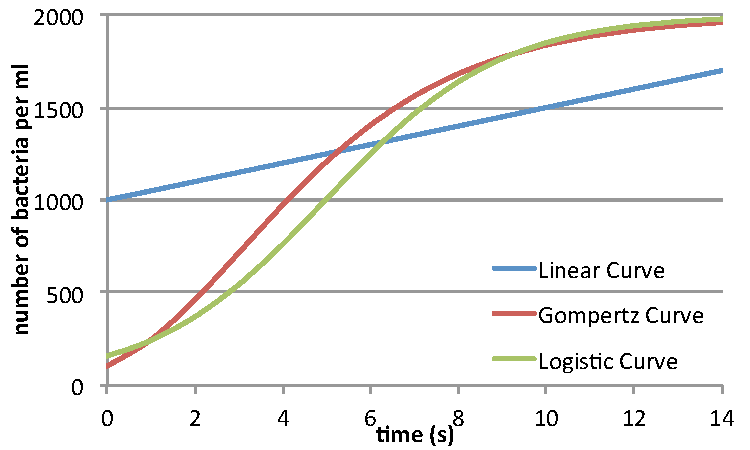
\includegraphics[height=3.5cm]{2_fig02}
\caption{Linear Curve, Gompertz Curve and Logistic Curve}
\vspace{-10pt}
\label{fig:growth_theory}
\end{figure}



\begin{figure*}[t!]
%\centering
\vspace{-10pt}
 \subfloat[CloudStack]{ 
    \label{fig:subfig:growth_dev_cloudstack}  
    \includegraphics*[width=0.53\columnwidth, viewport=0 0 370 250]{4_dev_growth_cloudstack}} 
 %\hspace{5pt}
 \subfloat[Eucalyptus]{ 
    \label{fig:subfig:growth_dev_eucalyptus}  
    \includegraphics*[width=0.5\columnwidth, viewport=20 0 370 250]{4_dev_growth_eucalyptus}} 
%  \hspace{5pt}
 \subfloat[OpenNebula]{ 
    \label{fig:subfig:growth_dev_opennebula}  
    \includegraphics*[width=0.5\columnwidth, viewport=18 0 370 250]{4_dev_growth_opennebula}} 
% \hspace{5pt}
 \subfloat[OpenStack]{ 
    \label{fig:subfig:growth_dev_openstack}  
    \includegraphics*[width=0.5\columnwidth, viewport=16 0 370 250]{4_dev_growth_openstack}} 
  \caption{The Growth of the Developer Communities} 
  \vspace{-15pt}
  \label{fig:growth_developer} 
\end{figure*}

\section{Growth Curves}
\label{sec:growth}

\subsection{Introduction to Growth Curves}

Growth curves have been applied in a wide range of disciplines, such as biology, fisheries, and medical science. Most organic matter grows with successive lag, exponential, stationary, and decline phases. A common characteristic of such growth curves is that growth is slowest at the start and end of a time period. A good example of such patterns is the growth of bacteria in a confined nutrient-containing broth, as shown in Figure \ref{fig:subfig:1a}. In the lag phase, bacteria become mature but are not yet able to reproduce. The exponential phase is characterized by cell doubling, where the number of new bacteria appearing per unit time is proportional to the present population. In the stationary phase, the growth rate is equal to the death rate, which is usually the result of nutrient depletion or spatial confinements. In the decline phase, bacteria run out of nutrient, and die. 


Bacteria exhibit multiple exponential growth phases under certain circumstances, which are called bi-phase growth or multi-phase growth, for example, when glucose and lactose are simultaneously present in the broth. The bacteria prefer to consume glucose, and will consume lactose only after the depletion of glucose. Since bacteria need some time to adapt to the new nutrient, the growth pauses and then resumes after a short period of time, resulting in the plateau between the two exponential growth phases. Bi-phase growth also occurs when nutrient is added to the broth when the growth has entered into decline phase, resulting in a second crest in the growth curve. Figure \ref{fig:subfig:1b} illustrates these two typical bi-phases growths.

A number of mathematical models have been proposed to represent such growth in the literature. Among these mathematical models, the Gompertz curve \cite{c5} and the logistic curve \cite{c6} – as shown in Figure \ref{fig:growth_theory} – have been adopted in a variety of disciplines. Examples of applications include bacteria growth in biology, tumor growth in medical science, population growth in social science, and market growth in economics. 

The formula for the Gompertz curve is

\begin{equation}
\label{eq:eqa}
\frac{dy}{dx} = \alpha y (ln y^{*} - ln y),
\end{equation}
or
\begin{equation}
\label{eq:eqb}
y = ye^{\alpha e^{\beta t}}.
\end{equation}

The formula for the logistic curve is
\begin{equation}
\label{eq:eqc}
\frac{dy}{dx} = \alpha y (y^{*} - y),
\end{equation}
or
\begin{equation}
\label{eq:eqd}
y = \frac{y^{*}}{1 + \alpha e^{\beta t} }.
\end{equation}


In Equations \ref{eq:eqa}, \ref{eq:eqb}, \ref{eq:eqc} and \ref{eq:eqd}, \textit{y*} represents the upper asymptote of the growth curves, while $\alpha$ is a parameter closely related to the growth rate. According to Equation \ref{eq:eqa}, the growth rate is a linear decreasing function of \textit{lny}. According to Equation \ref{eq:eqc}, the growth rate is a linear decreasing function of \textit{y}. As a result, in the stationary phase of the growth curves, the growth rate of the logistic curve decreases much faster than that of the Gompertz curve. Another major difference between these two growth curves is that the Gompertz curve is asymmetric, while the logistic curve is symmetric. The Gompertz curve reaches its maximum growth rate when \textit{y(t)} is 37\% of the upper asymptote, while the logistic curve reaches its maximum growth rate when \textit{y(t)} is 50\% of the upper asymptote. In Equations \ref{eq:eqb} and \ref{eq:eqd}, parameter $\beta$ determines the direction of the growth curves. The function grows when $\beta$ is negative, and declines when $\beta$ is positive. Both the Gompertz curve and the logistic curve work well in describing the lag, exponential, and stationary phases of normal growth. They are not applicable when the growth has entered the decline phase, nor are they suitable for describing bi-phase or multi-phase growths. 


The growth of open source communities is similar to the growth of bacteria in a confined nutrient-containing broth in that: (a) technology communities exhibit organic behavior in that the speed of technology diffusion is related to the current size of the community; (b) financial and human resources are needed to sustain the growth of the communities; and (c) there are growth limits for the communities due to technological, economical, social, and resource constrains. Therefore, growth curves established in other disciplines provide a solid basic on which we can study the growth of open source communities. 


\subsection{The Growth of Developer Communities}

The developer community of an open source project includes the developers who contribute code to the project. With the git version control system, developers usually identify themselves with their email addresses. In this study, we use email addresses associated with the commits to identity members of a developer community. When a developer makes a commit to an open source project, the developer becomes a members of the developer community of the project. However, a particular developer might stop contributing to this particular project at a certain point, upon which it is no longer appropriated to count this person as a member of the developer community. In this study, we use the concept of active contributors to describe the size of the developer communities, which include only the developers who have executed commit operations during a particular time interval. A developer community grows when the number of active contributors grows, and vice versa. 

 
Figure \ref{fig:growth_developer} shows the growths of the developer communities, as measured by the monthly number of active contributors. It should be noted that t(0) in these figures represents the month in which the project was launched. To account for the fluctuation in the collected data, we use a low pass filter to pre-process the data. The low pass filter we use is a moving average window filter, with the window size set to 3 months. Based on the filtered data, we use regression techniques to derive the key parameters of the growth curves for each developer community, and plot them on the same figure along with the filtered data. 

\begin{figure*}[t!]
%\centering
\vspace{-10pt}
 \subfloat[CloudStack]{ 
    \label{fig:subfig:growth_user_cloudstack}  
    \includegraphics*[width=0.53\columnwidth, viewport=0 0 370 250]{4_user_growth_cloudstack}} 
 \subfloat[Eucalyptus]{ 
    \label{fig:subfig:growth_user_eucalyptus}  
    \includegraphics*[width=0.53\columnwidth, viewport=18 0 370 250]{4_user_growth_eucalyptus}} 
  %\hspace{0.1in} 
 \subfloat[OpenNebula]{ 
    \label{fig:subfig:growth_user_opennebula}  
    \includegraphics*[width=0.48\columnwidth, viewport=18 0 370 250]{4_user_growth_opennebula}} 
 \subfloat[OpenStack]{ 
    \label{fig:subfig:growth_user_openstack}  
    \includegraphics*[width=0.48\columnwidth, viewport=16 0 370 250]{4_user_growth_openstack}} 
  \caption{The Growth of the User Communities} 
  \vspace{-15pt}
  \label{fig:growth_user} 
\end{figure*}

The growth of the CloudStack developer community (Figure 3a) fits relatively well with the growth curves except for the lag phase. CloudStack was originally developed by Cloud.com, but was later acquired by Citrix and donated to ASF. Before the acquisition and donation, CloudStack was developed by a core development team, but released as open source software, resulting in the flat line during the lag phase. After the donation, the project gained increasing level of attention from developers outside of Citrix, resulting in the exponential phase that fits well with the growth curves. This exponential phase stopped when the project graduated from Apache incubator and became a top level project of ASF. Currently the community is exhibiting characteristics of the decline phase, which can not be described by the growth curves.

The growth of the Eucalyptus developer community (Figure 3b) does not fit well with the growth curves and exhibits characteristics of a bi-phase growth. Eucalyptus got started as a university research project and had a stable development team before its first release. This is reflected by the flat line during the lag phase. The community entered an exponential phase starting from the 18th month, followed by a decline phase. The community entered a second exponential phase starting from the 37th month, followed by another decline phase. Both exponential phases exhibit linear behavior, suggesting that they are probably the result of planned hiring rather than unplanned organic grow. A closer look into the company's funding history reveals that the starting point of both exponential phases coincide with the time when the company received investments from venture capitals. In other words, these growth patterns are driven by the company’s internal business plan and hiring process, and thus exhibit only weak organic growth behavior.

The growth of the OpenNebula developer community (Figure 3c) seems to fit well with the growth curves except for the lag phase. However, this is a mis-perception because of insufficient data. The community has only 10 members at its peak, and maintains a stable size of 7 active contributors most of the time. This seems to be the size of the OpenNebula development team at C12G Labs, which does not change much over time. Similar to the case with Eucalyptus, the size of the OpenNebula developer community is driven by the company's internal business plan and hiring process, and does not exhibit organic growth behavior.  

The growth of the OpenStack developer community (Figure 3d) fits well with the growth curves. OpenStack got started as a community project with multiple founding organizations and is indicative of the importance and value of an extensive ecosystem. It spends significant amount of resources on persuading other organizations to join the ecosystem. As new organizations contribute developers to the project, they gradually dilute the influence of the founding members. With OpenStack, the number of active contributors does not depend on the business plan of any single organization, but depends on the collective resource being invested on the project by many organizations. Therefore, the OpenStack developer community exhibits characteristics of strong organic growth, and can be well represented by the growth curves. 


\subsection{The Growth of User Communities}

The user community of an open source project includes the people who use the open source software in various ways. Mailing lists and public forums are common discussion venues for open source user communities. In this study, members of a user community is defined as people participating in discussions by sending emails to mailing lists or posting messages to public forums. When a user sends an email to the mailing list or post a message to the public forum associated with an open source project, the user becomes a members of the user community of the project. However, a particular user might stop participating in community discussions at a certain point, upon which it is no longer appropriated to count this person as a member of the user community. In this study, we use the concept of active users to describe the size of the user communities, which include only the users who have participated in community discussions during a particular time interval. A user community grows when the number of active users grows, and vice versa. 

Figure \ref{fig:growth_user} shows the growths of the user communities, as measured by the monthly number of active users. Similar to the graphs for the developer communities, t(0) in these figures represents the month in which the project was launched. To account for the fluctuation in the collected data, we use a low pass filter to pre-process the data. The low pass filter we use is a moving average window filter, with the window size set to 3 months. Based on the filtered data, we use regression techniques to derive the key parameters of growth curves for each user community, and plot them on the same figure along with the filtered data. 

\begin{figure*}[t!]
\centering
%\vspace{-10pt}
 \subfloat[Monthly Number of Commits]{ 
    \label{fig:subfig:activity_commits}  
    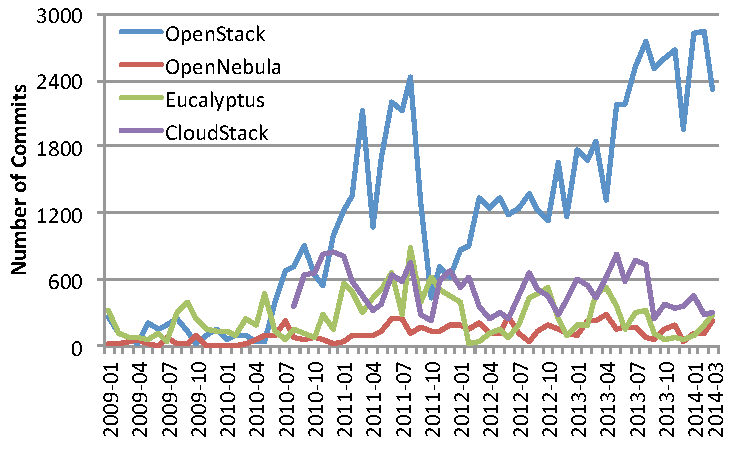
\includegraphics[height=4cm]{1_activity_commits}} 
  \hspace{50pt} 
 \subfloat[Monthly Number of Messages]{ 
    \label{fig:subfig:activity_messages}  
    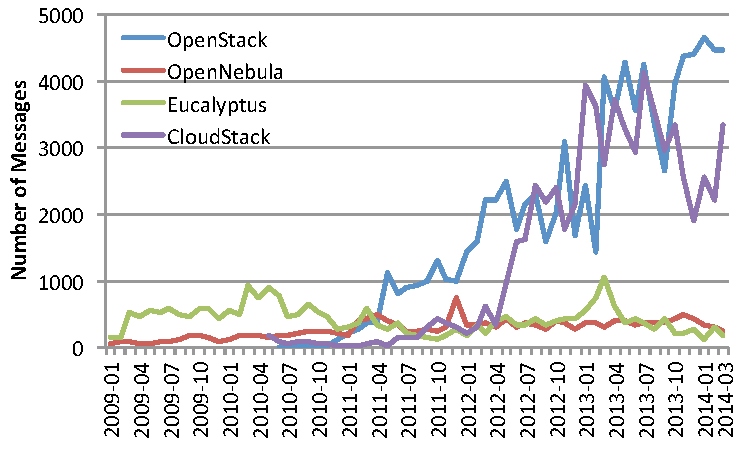
\includegraphics[height=4cm]{1_activity_messages}} 
  \caption{Developer and User Community Activities} 
  \vspace{-15pt}
  \label{fig:activities} 
\end{figure*}

The CloudStack project had a public forum and a mailing list from the very beginning. The forum and mailing list were replaced by several Apache incubator mailing lists when the project was donated to ASF. When the project became a top level project of ASF, the mailing lists were renamed to remove the incubator tag. The growth of the CloudStack user community (Figure 4a) fits well with the growth curves. The exponential phase started when the project was acquired by Citrix, and ended when the project became a top level project of ASF. Currently the community is exhibiting characteristics of the decline phase, that can't be described by growth curves. 

The Eucalyptus project had several changes make to its user community in the past. Originally the project had a mailing list and a public forum. The original forum was replaced by a new forum (Engage) in 2012, and the original mailing list was replaced by a Google group in 2013. In 2014 the new forum was terminated and all community discussions are now being directed to the Google group. Changes unfavorable to community growth is analogous to the removal of a nutrient from the broth, while changes favorable to community growth is analogous to the addition of nutrient to the broth. As a result, the The Eucalyptus user community exhibits typical bi-phase growth behavior (Figure 4b), which can not be described by the growth curves. The first exponential phase reached its peak when the project changed its open source license from Apache license to GPLv2. The second exponential phase started when the new forum was launched, and ended when the project began directing all community discussions to the Google group.

The OpenNebula project maintains a set of mailing lists for technical discussions on various topics. These discussion venues have not change over the past years. The growth of the OpenNebula user community fits well with the growth curves (Figure 4c). The community has exhibited characteristics of the stationary phase. 

The OpenStack project also maintains a set of mailing lists and public forums. Similar to the OpenNebula project, these discussion venues have not change over the past years. Similar to its developer community, the OpenStack user community also exhibits organic growth pattern, and fits well with the growth curves (Figure 4d). The user community is still in its exponential phase, with significant space to grow.


\section{Community Activities}
\label{sec:activity}

\subsection{Community Activity Metrics}

In this section, we study the volume of activities of the developer and user communities. For the developer communities, we use the number of git commits as an indicator of community activity. For the user communities, we use the number of messages - either an emails sent to a mailing list or posts published on a public forum - as an indicator of community activity. 

Figure \ref{fig:subfig:activity_commits} shows the volume of activities of the developer communities, as measured by the monthly number of commits. OpenStack has a much higher volume of commits than the other three projects. In the first quarter of 2014 Q1, on average there were 2500 commits make to OpenStack in every month. During the same period, CloudStack had about 350 commits per month, while Eucalyptus and OpenNebula had about 200 commits per month each. The primary reason for such huge difference in commits is that OpenStack is a collection of many component level sub-projects, while CloudStack, Eucalyptus and OpenNebula are standalone monolithic projects.    

Figure \ref{fig:subfig:activity_messages} shows the volume of activities of the user communities, as measured by the monthly number of messages. In 2009, Eucalyptus and OpenNebula began to gain the attention from cloud computing professionals. When CloudStack and OpenStack were introduced in the second half of 2010, some of the discussions moved from the Eucalyptus and OpenNebula user communities to the CloudStack and OpenStack user communities. As cloud computing continues to gain popularity, the volume of activities in the CloudStack and OpenStack user communities exhibits significant growth. However, such strong growth does not occur in the Eucalyptus and OpenNebula user communities. Currently, the volume of activities of the CloudStack and OpenStack user communities is much larger than the volume of activities of the Eucalyptus and OpenNebula user communities. In the first quarter of 2014, the OpenStack user community created approximately 3500 messages per month. During the same period, the monthly number of messages was 2500 for CloudStack, 300 for OpenNebula, and 150 for Eucalyptus. 


\begin{figure*}[t!]
\centering
 \subfloat[Developer Communities]{ 
    \label{fig:subfig:core_dev}  
    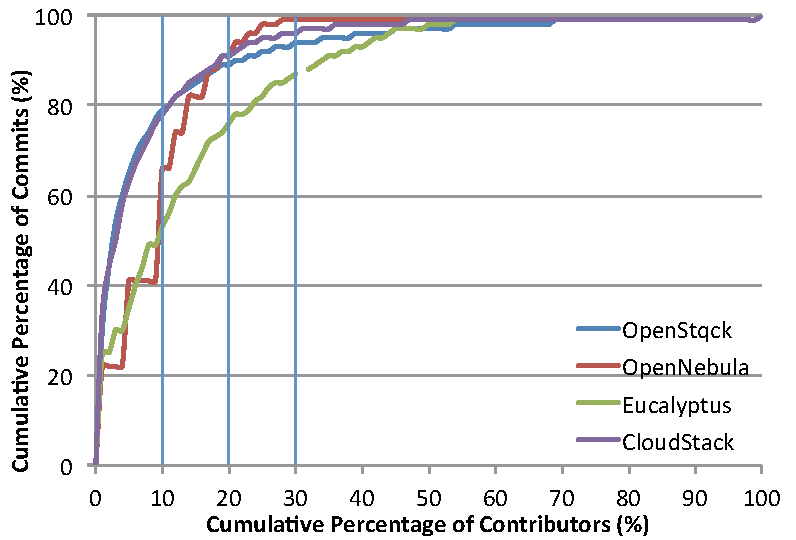
\includegraphics[width=6cm]{1_accumulated_dev}} 
  \hspace{50pt} 
 \subfloat[User Communities]{ 
    \label{fig:subfig:core_user}  
    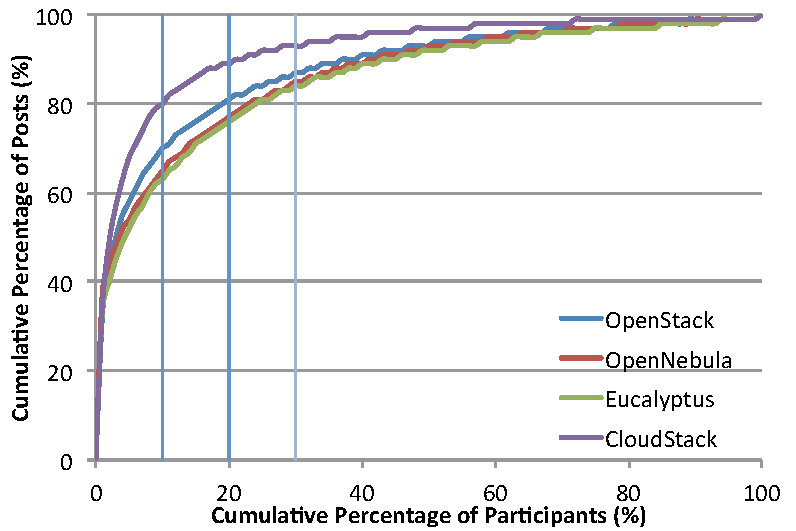
\includegraphics[width=6cm]{1_accumulated_user}} 
  \caption{The Contribution of Core Contributors} 
  \vspace{-10pt}
  \label{fig:core_contributor} 
\end{figure*}

\begin{figure*}[t!]
\centering
 \subfloat[Contributing Orgs. in Developer Communities]{ 
    \label{fig:subfig:org_dev}  
    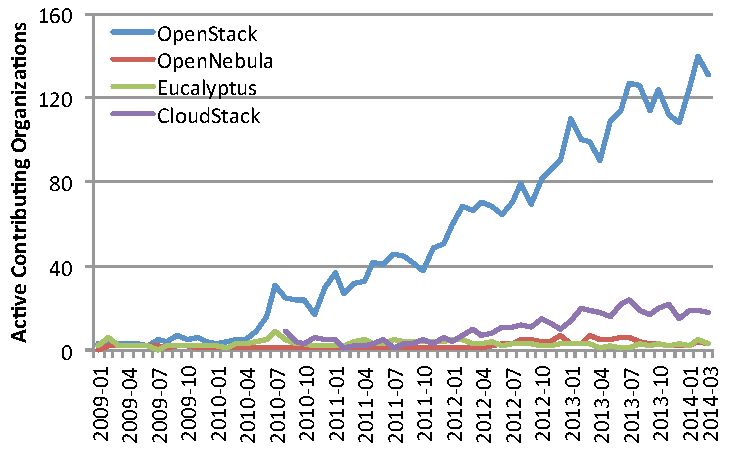
\includegraphics[width=6cm]{1_contrib_org_dev}} 
  \hspace{50pt} 
 \subfloat[Participating Orgs. in User Communities]{ 
    \label{fig:subfig:org_user}  
    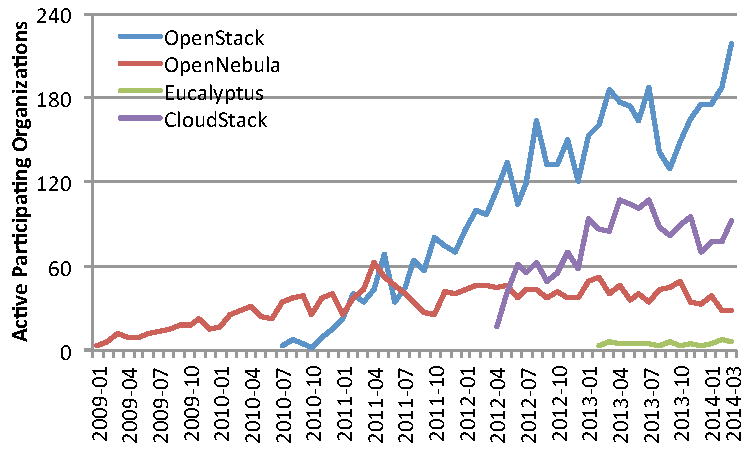
\includegraphics[width=6cm]{1_contrib_org_user}} 
  \caption{Organizational Participants} 
  \vspace{-10pt}
  \label{fig:org_contributor} 
\end{figure*}

\subsection{Core Contributors}

In a community there are usually a certain number of core members who have been involved with the community for a long time, and have make significant contributions to the community. In the context of open source developer communities, core members are people who contribute a significant portion of the code. In the context of open source user communities, core members are people leading discussions among mailing lists and public forums. In this section, we are more concerned about the relative size of the core members and the cumulative contributions they make to the community. 

Assuming that a community has a total number of \textit{n} members over its entire history, and the activities contributed by member \textit{M\textsubscript{i}} is \textit{A\textsubscript{i}}. Then the activities of the communities can be represented by a set \textit{A = \{A\textsubscript{1}, A\textsubscript{2}, ..., A\textsubscript{n}\}}, where members of set \textit{A} is sorted in a descending order. The top x\% core members includes \textit{m} members, where \textit{m} is defined as
\begin{equation}
\label{eq:top_m_members}
m = (ceil) \frac{ 100x }{n}.
\end{equation}
The cumulative contributions make by the core members can be calculated by the cumulative distribution function (CDF):
\begin{equation}
\label{eq:top_m_contributions}
y = \frac{100 \sum_{i=1}^{i=m} A_{i}}{\sum_{i=1}^{i=n} A_{i}},
\end{equation}
\\where y is the percentage of contributions make by the top x percentage of core members. 

Figure \ref{fig:core_contributor} shows the cumulative percentage of members, as against the cumulative percentage of contributions they make, for the developer and user communities. A simple way to read these figures is x\% of core members contribute y\% of the activities in the community. These curves exhibit characteristic of the power law distribution, with a few that dominate to the left and the long tail to the right. For the developer communities, the contributions make by the top 10\% core members are 80\%, 53\%, 66\%, 80\% for CloudStack, Eucalyptus, OpenNebula and OpenStack.  For the user communities, the contributions make by the top 10\% core members are 80\%, 63\%, 65\%, and 70\% for CloudStack, Eucalyptus, OpenNebula and OpenStack. 

\begin{table*}[t!]
\caption{Top 10 Contributing Domains in the Developer Communities in 2014 Q1}
\label{tbl:dev}
\centering
\begin{tabular}{|c|c|c|c|c|c|c|c|} \hline
    \multicolumn{2}{|c|}{CloudStack} &
    \multicolumn{2}{|c|}{Eucalyptus} &
    \multicolumn{2}{|c|}{OpenNebula} &
    \multicolumn{2}{|c|}{OpenStack} \\ \hline
citrix.com & 38\% & eucalyptus.com & 86\% & opennebula.org & 92\% & redhat.com & 16\% \\ \hline
    gmail.com & 17\% & gmail.com & 12\% & c12g.com & 5\% & gmail.com & 14\% \\ \hline
	schubergphilis.com & 8\% & devzero.com & 1\% & other & 3\% & ibm.com & 9\% \\ \hline
	apache.org & 7\% & other & 1\% & & & openstack.org & 6\% \\ \hline
	cloud.com & 6\% & & & & & hp.com & 5\% \\ \hline
	onecht.net & 4\% & & & & & mirantis.com & 4\% \\ \hline
	solidfire.com & 3\% & & & & & suse.de & 4\% \\ \hline
	clogeny.com & 2\% & & & & & enovance.com & 3\% \\ \hline
	widodh.nl & 1\% & & & & & rackspace.com & 2\% \\ \hline
	other & 14\% & & & & & intel.com & 2\% \\ \hline
	 &  & & & & & other & 33\% \\ \hline
\end{tabular}
\end{table*}

\begin{table*}[t!]
\caption{Top 10 Contributing Domains in the User Communities in 2014 Q1}
\label{tbl:user}
\centering
\begin{tabular}{|c|c|c|c|c|c|c|c|} \hline
    \multicolumn{2}{|c|}{CloudStack} &
    \multicolumn{2}{|c|}{Eucalyptus} &
    \multicolumn{2}{|c|}{OpenNebula} &
    \multicolumn{2}{|c|}{OpenStack} \\ \hline
    gmail.com & 38\% & gmail.com & 56\% & opennebula.org & 33\% & gmail.com & 23\% \\ \hline
    citrix.com & 18\% & eucalyptus.com & 35\% & gmail.com & 19\% & redhat.com & 11\% \\ \hline
	apache.org & 15\% & fedoraproject.org & 2\% & c12g.com& 7\% & mirantis.com & 9\% \\ \hline
	outlook.com & 4\% & passur.com & 2\% & bit.nl & 6\% & rackspace.com & 4\% \\ \hline
	microsoft.com & 1\% & openida.com & 1\% & yahoo.com & 4\% & ibm.com & 3\% \\ \hline
	shapeblue.com & 1\% &di.unipmn.it & 1\% & baby-gnu.org& 3\% & openstack.org & 3\% \\ \hline
	stratesec.co & 1\% & other & 3\% & fnal.gov& 2\% & dague.net & 3\% \\ \hline
	qq.com & 1\% & & & scss.tcd.ie& 2\% & dreamhost.com & 2\% \\ \hline
	163.com & 1\% & & & msn.com& 1\% & hp.com & 2\% \\ \hline
	cloudops.com & 1\% & & & vrt.com.au& 1\% & robertcollins.com & 2\% \\ \hline
	other & 19\% & & & other& 22\% & other &36\% \\ \hline
\end{tabular}
\end{table*}


\begin{table*}[t!]
\caption{Diversity of the Developer and User Communities in 2014 Q1}
\label{tbl:diversity}
\centering
\begin{tabular}{|c|c|c|c|c|c|c|c|c|} \hline
    \multicolumn{1}{|c|}{} &
    \multicolumn{4}{|c|}{Developer Communities} &
    \multicolumn{4}{|c|}{User Communities} \\ \hline
	  & diversity index & growth curves & upper asymptote & growth phase & diversity index & growth curves & upper asymptote & growth phase \\ \hline
	 CloudStack & 0.2108 & Partial Fit & 110 & decline & 0.2376 & Fit Well & 350 & decline \\ \hline
	 Eucalyptus & 0.7542 & Not Fit & 50 & bi-phase & 0.4379 & Not Fit & 200 & bi-phase \\ \hline
	 OpenNebula & 0.8498 & Not Fit & 10 & stationary & 0.2054 & Fit Well & 80 & stationary \\ \hline
	 OpenStack  & 0.1732 & Fit Well & 1000 & exponential & 0.2082 & Fit Well & 1500 & exponential \\ \hline
\end{tabular}
\end{table*}


\section{Diversity of Community}
\label{sec:diversity}

In Section \ref{sec:growth}, we made the assertion that the Eucalyptus and OpenNebula developer communities are driven by their internal business plans and hiring processes. To examine the validity of such an assumption, we need to investigate which are the organizations that contribute code to these open source projects and that participate in discussions in the user communities. In this study, we identify the organizations to which a user or developer belongs to by the domain name in his/her email address. Similar to the concept of active contributors and active participants in the developer and user communities, a particular organization might stop participating in a particular developer or user community at a certain point, upon which it is no longer appropriate to be counted as a contributing organization. In this study, we use the concept of active participating organizations to describe the organization contributing code or participating in community discussions during a particular time interval.


Figure \ref{fig:subfig:org_dev} shows the monthly number of active contributing organizations for the developer communities. OpenStack has the largest number of active contributing organizations, and the number of active contributing organizations is growing in a near-linear fashion. CloudStack also has quite a few active contributing organizations, but the number seems to stop growing since 2013 Q1. Eucalyptus and OpenNebula have only very few active contributing organizations, and the numbers are not growing. Table \ref{tbl:dev} shows the top ten actively contributing domains for the developer communities in 2014 Q1, ranked by the percentage of commits they made to each project during that quarter. As shown in the table, multiple organizations jointly contribute to CloudStack, but Citrix still plays a very important role in the community. The combined contribution from citrix.com and cloud.com represents 44\% of the commits. OpenStack is also jointly contributed to by multiple organizations, but none of these organizations are in a dominant position to control the community. Eucalyptus and OpenNebula are both projects dominated by a single organization, with almost no contribution from the community. These observations confirm that the growth of the CloudStack and OpenStack developer communities are driven by the communities, while the growths of the Eucalyptus and OpenNebula developer communities are driven by a single organization's internal business plans and hiring processes.

Figure \ref{fig:subfig:org_user} shows the monthly number of active participating organizations for the user communities. For this particular analysis, we only included data from the mailing lists because public forums do not disclose email addresses of the registered users. OpenStack has the largest number of actively participating organizations, followed by CloudStack and OpenNebula. However, the difference in the number of participating organizations is not as big as the difference in the developer communities. Table \ref{tbl:dev} shows the top 10 participating domains for the developer communities in 2014 Q1, ranked by the percentage of messages they sent to the mailing lists during that quarter. As shown in the table, the user communities of CloudStack, OpenNebula and OpenStack include a diversity of participating organizations. The user community of Eucalyptus has only very few participating organizations.

The diversity of a community can be represented by Simpson's diversity index \cite{c7}, which can be calculated by the following equation:
\begin{equation}
\label{eq:diversity}
D=\sum_{i=0}^{i=n} p_{i}^{2},
\end{equation}
\\where \textit{D} is Simpson's diversity index, \textit{n} is the number of organizations in the community, while \textit{p\textsubscript{i}} represents the contribution from the \textit{i\textsuperscript{th}} organization. When the Simpson's diversity index is 0, the community has infinite diversity. When the Simpson's diversity index is 1, the community has no diversity. That is, the smaller the value \textit{D}, the greater the diversity. 

We used the data from Table \ref{tbl:dev} and Table \ref{tbl:user} to calculate the Simpson's diversity index. Table \ref{tbl:diversity} shows the diversity index of the developer and user communities, as well as how they fit with the growth curves, the upper asymptote of the growth curves, and the growth phase they are in. As shown in the table, communities with greater diversity exhibit closer-to-organic growth behavior and fit better with the growth curves. The upper asymptote of the growth curves represents the theoretical maximum size of the communities. As we can see, communities with greater diversity have greater upper asymptote, and are usually larger in terms of active members. 


\section{Related Work}
\label{sec:related}

In recent years, open source software have received increasing level of attention from the academic community. Extensive literature exists on what open source software is \cite{g1}, economical considerations such as intellectual property and personal motivation \cite{g2}, how individual and organizations join and contribute to open source projects \cite{g3}, as well as the impact of community participation on the performance of commercial companies \cite{g4}. Most of these researche papers have adopted a methodology that is qualitative rather than quantitative, and it is difficult to generalize the result. 

Godfrey et al. \cite{c9} investigated the evolution of open source software, using the Linux kernel as a case study. They analyzed the various releases of the Linux kernel source code between 1993 to 2001, using the gzip compressed size and lines of code to measure the growth of the Linux kernel project. They found that the Linux kernel project was growing in a linear fashion, which was surprising in that previously published research had suggested that large software systems tended to grow slower as they became larger. 

Mockus et al. \cite{c10} investigated the growth of the Apache web server project and the Mozilla web browser project, using email archives of source code change history and problem reports. They quantitatively studied aspects such as developer participation, core team size, code ownership, productivity, defect density, and bug resolution intervals for these two projects, and compared them with several commercial projects. The authors further proposed that a commercial/open source hybrid would yield in high-performance software development process. 

Oh et al. \cite{c11} investigated the interaction patterns among OSS community members, as well as the impact of size and connectivity on the stability of an OSS network. Their computer simulation results indicated that membership herding is negatively related to external influences and tends to occur in large networks with random connectivity. 

Huang et al. \cite{c12} analyzed the structure and evolution of the Drupal content management system. The techniques they employed include social network analysis, degree distribution, hierarchical clustering, and scientific visualization. They reported that structure of the Drupal community displayed scale-free characteristics, which have been observed in a large number of other social, technical and biological networks. 

\section{Conclusion}
\label{sec:conclusion}

In this paper, we study the growth of the developer and user communities of four major open source projects in the area of Infrastructure- as-a-Service (IaaS). The contributions of this paper include:

1. We measured the size these communities using with active contributors / participants. We modeled the growth of these communities with the Gompertz curve and the logistic curve. The CloudStack and OpenStack developer communities exhibit characteristics of organic growth and fit well with the growth curves. The Eucalyptus and OpenStack developer communities are driven by their internal business plans, therefore do not fit well with the growth curves. The CloudStack, OpenNebula and OpenStack user communities exhibit characteristics of organic growth, and fit well with the growth curves. The Eucalyptus user communities exhibits bi-phase growth behavior, and does not fit with the growth curves.

2. We measured the activities of these communities using git commits and messages posted to mailing lists and public forums. We found that a small group of core contributors contribute the majority of the activities. For the developer communities, contributions make by the top 10\% core members are 80\%, 53\%, 66\%, 80\% for CloudStack, Eucalyptus, OpenNebula and OpenStack. For the user communities, contributions make by the top 10\% core members are 80\%, 63\%, 65\%, and 70\% for CloudStack, Eucalyptus, OpenNebula and OpenStack. 

3. We measured the number of active contributing organizations for these communities. We evaluated the diversity of these communities using Simpson’s diversity index. Communities with greater diversity exhibit closer-to-organic growth behavior and fit better with the growth curves. Further more, communities with greater diversity are usually larger in terms of active members.

The main limitation of this paper is the small size of the sample. The results obtained suggest an interesting connection between diversity and growth. This hypothesis is not yet ready to be generalized to open source communities in other problem domains. In our future studies, we will test this hypothesis using a bigger sample of open source communities in order to arrive at a more generalisable result on the relationship between organizational diversity and growth of the communities.


\begin{thebibliography}{1} 

\bibitem{nist}
Peter Mell, Timothy Grance, Definition of Cloud Computing, Special Publication 800-145, National Institute of Standards and Technology, 2011

\bibitem{c1}
D. Nurmi, R. Woski, C. Grzegorczyk, G. Obertelli, S. Soman, L. Youseff, D. Zagorodnov, “The Eucalyptus Open-Source Cloud-Computing System”, Proc. 9th IEEE International Symposium on Cluster Computing, pp. 124-131, May 2009

\bibitem{c2}
M. Dejan, I. M. LIorente, R. S. Montero, “OpenNebula: A Cloud Management Tool”, Internet Computing, IEEE, vol. 15, issue 2, pp. 11-14, March-April 2011

\bibitem{c3}
Keith Shackelford, James Williams, “Infrastructure as a Service (IaaS) for NASA’s Mission Directorate, NASA’s Nebula Pioneers a New Frontier for Cloud Computing”, 2012 International Conference on Computing, Networking and Communications (ICNC), pp. 29-33, February 2012

\bibitem{c4}
Subhash Saini, Steve Heistand, Haoqiang Jin, Johnny Chang, Robert Hood, Piyush Mehrotra, Rupak Biswas, “An Application-Based Performance Evaluation of NASA’s Nebula Cloud Computing Platform”, 2012 IEEE 14th International Conference on High Performance Computing and Communications, pp. 336-343, June 2012

\bibitem{c5}
Charles P. Winson, “The Gompertz Curve as a Growth Curve”, Proceedings of the National Academic of Science, vol. 18, no. 1, pp. 1-8, 1932 

\bibitem{c6}
M. H. Zwietering, I. Jongenburger, F. M. Rombouts, K. Van’t Riet, “Modeling of the Bacterial Growth Curve”, Applied and Environmental Microbiology, vol. 56, no. 6, pp. 1875-1881, 1990

\bibitem{c7}
Edward H. Simpson, "Measurement of Diversity." Nature, 1949

\bibitem{g1}
Eric Raymond, "The Cathedral and the Bazaar", Knowledge, Technology and Policy, vol. 12, no. 3, pp. 23-49, 1999

\bibitem{g2}
Bruce Kogut, Anca Metiu, "Open-Source Software Development and Distributed Innovation", Oxford Review of Economic Policy, vol. 17, no. 2, pp. 248-264, 2001

\bibitem{g3}
Georg von Krogh, Sebastian Spaeth, Karim R. Lakhani, "Community, Joining, and Specialization in Open Source Software Innovation", Research Policy, vol. 32, no. 7, pp. 1217-1241, 2003

\bibitem{g4}
Wouter Stam, "When Does Community Participation Enhance the Performance of Open Source Software Companies?", Research Policy, vol. 38, no. 8, pp. 1288-1299, 2009 

\bibitem{c9}
Michael W. Godfrey, Qiang Tu, “Evolution in Open Source Software: A Case Study”, Proceedings of 2000 International Conference on Software Maintenance, pp. 131-142, IEEE Press, 2000

\bibitem{c10}
Audris Mockus, Roy T. Fielding, James D. Herbsleb, “Two Case Studies of Open Source Software Development: Apache and Mozilla”, ACM Transactions on Software Engineering and Methodology, vol. 11, no. 3, pp. 309-346, 2002

\bibitem{c11}
Wonseok Oh, Sangyong Jeon, "Membership Herding and Network Stability in the Open Source Community: The Ising Perspective", Management Science, vol. 53, no. 7, pp. 1086-1101, 2007

\bibitem{c12}
Hao-Yun Huang, Qize Le and Jitesh H. Panchal, "Analysis of the Structure and Evolution of An Open-Source Community", Journal of Computing and Information Science in Engineering, vol. 11, no. 3, 2011

\end{thebibliography}


\end{document}